% A LaTeX (non-official) template for ISAE projects reports
% Copyright (C) 2014 Damien Roque
% Version: 0.2
% Author: Damien Roque <damien.roque_AT_isae.fr>

\documentclass[a4paper,12pt,calibri,oneside,openany]{book}
\usepackage{geometry}
\usepackage[utf8]{inputenc}
\usepackage[T1]{fontenc}
\usepackage[french]{babel} % If you write in French
%\usepackage[english]{babel} % If you write in English
\usepackage{a4wide}
\usepackage{graphicx}
\graphicspath{{images/}}
\usepackage{subfig}
\usepackage{tikz}
\usetikzlibrary{shapes,arrows}
\usepackage{pgfplots}
\pgfplotsset{compat=newest}
\pgfplotsset{plot coordinates/math parser=false}
\newlength\figureheight
\newlength\figurewidth
\pgfkeys{/pgf/number format/.cd,
set decimal separator={,\!},
1000 sep={\,},
}
\usepackage{ifthen}
\usepackage{ifpdf}
\ifpdf
\usepackage[pdftex]{hyperref}
\else
\usepackage{hyperref}
\fi
\usepackage{color}
\hypersetup{%
colorlinks=true,
linkcolor=black,
citecolor=black,
urlcolor=black}
\usepackage{float}
\renewcommand{\baselinestretch}{1.05}
\usepackage{fancyhdr}
\pagestyle{fancy}
\fancyfoot{}
\fancyhead[LE,RO]{\bfseries\thepage}
\fancyhead[RE]{\bfseries\nouppercase{\leftmark}}
\fancyhead[LO]{\bfseries\nouppercase{\rightmark}}
\setlength{\headheight}{15pt}

\let\headruleORIG\headrule
\renewcommand{\headrule}{\color{black} \headruleORIG}
\renewcommand{\headrulewidth}{1.0pt}
\usepackage{colortbl}
\arrayrulecolor{black}

\fancypagestyle{plain}{
  \fancyhead{}
  \fancyfoot[C]{\thepage}
  \renewcommand{\headrulewidth}{0pt}
}

\makeatletter
\def\@textbottom{\vskip \z@ \@plus 1pt}
\let\@texttop\relax
\makeatother

\makeatletter
\def\cleardoublepage{\clearpage\if@twoside \ifodd\c@page\else%
  \hbox{}%
  \thispagestyle{empty}%
  \newpage%
  \if@twocolumn\hbox{}\newpage\fi\fi\fi}
\makeatother

\newcommand{\mycontour}[1]{%
	\contour{red}{#1}%
}

\newcommand{\myuline}[1]{%
	\uline{\phantom{#1}}%
	\llap{\contour{white}{#1}}%
}


\usepackage{amsthm}
\usepackage{amssymb,amsmath,bbm}
\usepackage{array}
\usepackage{bm}
\usepackage{multirow}
\usepackage[footnote]{acronym}
\usepackage{float}
\usepackage{wasysym}
\usepackage{wrapfig}
\usepackage{url}
\usepackage{eurosym}
\usepackage{array}
\usepackage{xcolor}
\usepackage{supertabular}
%\usepackage{geometry}
\usepackage{pdflscape}
\usepackage{calrsfs}
\usepackage{minted}
\newcommand*{\SET}[1]  {\ensuremath{\mathbf{#1}}}
\newcommand*{\VEC}[1]  {\ensuremath{\boldsymbol{#1}}}
\newcommand*{\FAM}[1]  {\ensuremath{\boldsymbol{#1}}}
\newcommand*{\MAT}[1]  {\ensuremath{\boldsymbol{#1}}}
\newcommand*{\OP}[1]  {\ensuremath{\mathrm{#1}}}
\newcommand*{\NORM}[1]  {\ensuremath{\left\|#1\right\|}}
\newcommand*{\DPR}[2]  {\ensuremath{\left \langle #1,#2 \right \rangle}}
\newcommand*{\calbf}[1]  {\ensuremath{\boldsymbol{\mathcal{#1}}}}
\newcommand*{\shift}[1]  {\ensuremath{\boldsymbol{#1}}}

\newcommand{\eqdef}{\stackrel{\mathrm{def}}{=}}
\newcommand{\argmax}{\operatornamewithlimits{argmax}}
\newcommand{\argmin}{\operatornamewithlimits{argmin}}
\newcommand{\ud}{\, \mathrm{d}}
\newcommand{\vect}{\text{Vect}}
\newcommand{\sinc}{\ensuremath{\mathrm{sinc}}}
\newcommand{\esp}{\ensuremath{\mathbb{E}}}
\newcommand{\hilbert}{\ensuremath{\mathcal{H}}}
\newcommand{\fourier}{\ensuremath{\mathcal{F}}}
\newcommand{\sgn}{\text{sgn}}
\newcommand{\intTT}{\int_{-T}^{T}}
\newcommand{\intT}{\int_{-\frac{T}{2}}^{\frac{T}{2}}}
\newcommand{\intinf}{\int_{-\infty}^{+\infty}}
\newcommand{\Sh}{\ensuremath{\boldsymbol{S}}}
\newcommand{\C}{\SET{C}}
\newcommand{\R}{\SET{R}}
\newcommand{\Z}{\SET{Z}}
\newcommand{\N}{\SET{N}}
\newcommand{\K}{\SET{K}}
\newcommand{\reel}{\mathcal{R}}
\newcommand{\imag}{\mathcal{I}}
\newcommand{\cmnr}{c_{m,n}^\reel}
\newcommand{\cmni}{c_{m,n}^\imag}
\newcommand{\cnr}{c_{n}^\reel}
\newcommand{\cni}{c_{n}^\imag}
\newcommand{\tproto}{g}
\newcommand{\rproto}{\check{g}}
\newcommand{\LR}{\mathcal{L}_2(\SET{R})}
\newcommand{\LZ}{\ell_2(\SET{Z})}
\newcommand{\LZI}[1]{\ell_2(\SET{#1})}
\newcommand{\LZZ}{\ell_2(\SET{Z}^2)}
\newcommand{\diag}{\operatorname{diag}}
\newcommand{\noise}{z}
\newcommand{\Noise}{Z}
\newcommand{\filtnoise}{\zeta}
\newcommand{\tp}{g}
\newcommand{\rp}{\check{g}}
\newcommand{\TP}{G}
\newcommand{\RP}{\check{G}}
\newcommand{\dmin}{d_{\mathrm{min}}}
\newcommand{\Dmin}{D_{\mathrm{min}}}
\newcommand{\Image}{\ensuremath{\text{Im}}}
\newcommand{\Span}{\ensuremath{\text{Span}}}

\newcommand{\anfr}[1]{{\bfseries\underline{#1}}}

\newtheoremstyle{break}
  {11pt}{11pt}%
  {\itshape}{}%
  {\bfseries}{}%
  {\newline}{}%
\theoremstyle{break}

%\theoremstyle{definition}
\newtheorem{definition}{Définition}[chapter]

%\theoremstyle{definition}
\newtheorem{theoreme}{Théorème}[chapter]

%\theoremstyle{remark}
\newtheorem{remarque}{Remarque}[chapter]

%\theoremstyle{plain}
\newtheorem{propriete}{Propriété}[chapter]
\newtheorem{exemple}{Exemple}[chapter]



%\sloppy
\usepackage{wrapfig}
\usepackage{enumitem}
\usepackage{pifont}
\usepackage{makeidx}
\usepackage{setspace}
\makeindex
\usepackage[xindy]{glossaries}
\makeglossaries
%\loadglsentries{glossaire.tex}




\begin{document}

\renewcommand{\bibname}{Bibliographie et Webographie}
%%%%%%%%%%%%%%%%%%
%%% First page %%%
%%%%%%%%%%%%%%%%%%

\begin{titlepage}
\begin{center}


\includegraphics[width=0.6\textwidth]{ipsa}\\[1cm]

{\large Étudiants ingénieurs en aérospatial}\\[0.5cm]

{\large Mémoire de 3\up{e} année}\\[0.5cm]

% Title
\rule{\linewidth}{0.5mm} \\[0.4cm]
{ \huge \bfseries Théorie et Benchmark des méthodes de descente en vue d'une application au machine learning\\[0.4cm] }
\rule{\linewidth}{0.5mm} \\[1.5cm]

% Author and supervisor
\noindent
\begin{minipage}{0.4\textwidth}
  \begin{flushleft} \large
    \emph{Auteurs :}\\
    M. \bsc{Audet} Yoann\\
    M. \bsc{Chandon} Clément\\
    M. \bsc{De Claverie} Chris\\
    M. \bsc{Huynh} Julien
  \end{flushleft}
\end{minipage}%
\begin{minipage}{0.4\textwidth}
  \begin{flushright} \large
    \emph{Encadrant :} \\
    Pr. \bsc{Peschard} Cédric\\
  \end{flushright}
\end{minipage}

\vfill

% Bottom of the page
{\large Version 1.0 du\\ \today}

\end{center}
\end{titlepage}

%%%%%%%%%%%%%%%%%%%%%%%%%%%%%
%%% Non-significant pages %%%
%%%%%%%%%%%%%%%%%%%%%%%%%%%%%

\frontmatter

\chapter*{Remerciements}

\tableofcontents

\mainmatter
\pagestyle{fancy}
%%%%%%%%%%%%%%%%%%%%%%%%%%%%%%%%%%%%%%%%%%%%
%%% Content of the report and references %%%
%%%%%%%%%%%%%%%%%%%%%%%%%%%%%%%%%%%%%%%%%%%%



\chapter{Introduction}
\chapter{Développement théorique des méthodes de descente}

Le but de ce rapport est d'étudier les différentes possibilités afin de minimiser une fonction. Le problème se formule de la manière suivante : 
\begin{equation}
\argmin_x f(x)
\end{equation}

Nous utiliserons des méthodes de descente afin de résoudre ce type de problème mais avant tout, il est nécessaire de définir l'intérêt de résoudre un tel type de problème puis de l'encadrer.

%%%%%%%%%%%%%%%%%%%%%%%%%%%%%%%%%%%%%%%%%%%%%%%%%%%%%%%%%%%%
% 				METHODES DE DESCENTES
%%%%%%%%%%%%%%%%%%%%%%%%%%%%%%%%%%%%%%%%%%%%%%%%%%%%%%%%%%%%
\section{Retour sur les méthodes de descente}
\subsection{Motivation de l'étude et de l'intérêt}
Lorsque nous traitons d'optimisation, la fonction dont nous cherchons généralement l'$\argmin$, est une fonction objectif. Ces fonctions à minimiser sont présentes dans de nombreux domaines très différents dont l'économie, la mécanique, la production industrielle ou dans la gestion de flux et de réseaux. Les applications sont nombreuses. Il est donc important de pouvoir trouver des méthodes efficaces de résolution de ce problème général. 
\subsection{Encadrement du problème}
On cherche donc l'argument $x$ tel que $f(x)$ soit minimal, $f$ étant une fonction deux fois différentiable sur $\mathbb{R}^n$. On se donne deux conditions essentielles car sans celles-ci, l'étude devient beaucoup plus complexe. \\

On pose donc que la fonction $f$ que l'on cherche à minimiser est une fonction strictement convexe afin d'utiliser les outils de l'analyse convexe. De plus, on suppose que $f$ est coercive sur l'ensemble d'étude $R^n$. Mathématiquement, ces deux conditions se traduisent par :
$$
\forall t \in ]0;1[, \forall (x,y) \in \mathbb{R}^2, x\neq y, f(tx+(1-t)y)<tf(x)+(1-t)f(y) 
$$
\begin{center}
	et
\end{center}
$$
\lim\limits_{|x|\rightarrow +\infty}f(x)=+\infty
$$

La coercivité permet d'assurer l'existence d'une solution et la stricte convexité de limiter le nombre de solution à une, au plus. En posant ces deux conditions, notre problème d'optimisation aura une solution unique que l'on notera $x^*$.

\subsection{Intérêt d'une fonction $\mathcal{C}^2$ sur $\mathbb{R}^n$}
Dans ce mémoire nous nous intéressons uniquement aux fonctions objectif qui sont deux fois différentiables sur $\mathbb{R}^n$ et de classe $\mathcal{C}^2$. \\

Cela a son importance puisque dans bon nombre de cas, nous effectuerons un développement limité sur la fonction $f$, localement, afin d'obtenir une forme quadratique plus un reste qui dépendra du choix que nous effectuerons (Reste de Young, reste intégral ou reste de Taylor-McLaurin). \\

Notre problème d'optimisation différentiable se rapprochera donc d'un problème de minimisation quadratique et nous pourrons ainsi trouver un minimiseur local qui, dans le cadre d'une fonction strictement convexe et coercive, sera le minimum global unique recherché.
\subsection{Les méthodes de gradients}
Les méthodes de gradients sont des méthodes de descentes basées sur la connaissance du gradient de la fonction objectif. Nous verrons trois méthodes de descente de gradient classiques qui sont :
\begin{enumerate}
	\item Le gradient à pas fixe
	\item Le gradient à pas optimal
	\item Le gradient conjugué
\end{enumerate}
\subsubsection{Principes}
L'idée derrière ces méthodes est de trouver $\argmin_x f(x)$ à partir d'un point initial puis d'en choisir une direction et un pas de descente. L'efficacité de l'algorithme sera grandement influencée par le pas de descente. Le choix de ce paramètre donne naissance aux trois méthodes que nous étudions.
\subsubsection{Méthode du gradient à pas fixe}
La méthode du gradient à pas fixe est la plus simple à mettre en place. Cependant, elle peut être dangereuse puisque l'on peut se dire qu'un pas très grand permettra d'atteindre la solution recherchée plus rapidement. Cela induit en erreur puisque dans un tel cas (grand pas), il est possible d'osciller autour de la solution sans jamais l'atteindre à un seuil de précision convenable. L'algorithme est le suivant :
\begin{algorithm}
	\caption{Méthode du gradient à pas fixe}
	\begin{algorithmic}[1]
		\Procedure{Méthode du gradient à pas fixe}{$x_0,n_{Max},\rho$}
		\State Soit $i=1$
		\While{$||\nabla f(x^{(i)})||>tol\ \& \ i<n_{Max}$}
		\State $d^{(i)}=-\nabla f(x^{(i)})$;
		\State $x^{(i+1)}=x^{(i)}+\rho d^{(i)}$;
		\State $i = i+1$;
		\EndWhile
		\EndProcedure
	\end{algorithmic}
\end{algorithm}
\subsubsection{Méthode du gradient à pas optimal}
Une manière d'améliorer les performances de l'algorithme serait d'y faire une recherche de pas optimal à chaque itération.
\begin{algorithm}[H]
	\caption{Méthode du gradient à pas  optimal}
	\begin{algorithmic}[1]
		\Procedure{Méthode du gradient à pas  optimal}{$x_0,n_{Max},\rho_0$}
		\State Soit $i=1$
		\While{$||\nabla f(x^{(i)})||>tol\ \& \ i<n_{Max}$}
		\State $d^{(i)}=-\nabla f(x^{(i)})$;
		\State $\rho^{(i)}=rechercheduPas(x^{(i)},d^{(i)},\rho_0,tolR)$
		\State $x^{(i+1)}=x^{(i)}+\rho^{(i)} d^{(i)}$;
		\State $i = i+1$;
		\EndWhile
		\EndProcedure
	\end{algorithmic}
\end{algorithm}
L'algorithme de recherche du pas est :
\begin{algorithm}[H]
	\caption{Recherche du pas inexact}
	\begin{algorithmic}[1]
		\Procedure{Recherche du pas inexact}{$x^{(i)},d^{(i)},\rho_0,tolR$}
		\State Soit $j=1$, $\rho^{(0)}=10\rho^{(1)}$
		\While{$||\rho^{(j)}-\rho^{(j-1)}||>tolR\ \&\ j<maxIt$}
		\State $\varphi^{'}(\rho^{(j)})=d^{(i)^T}\nabla f(x^{(i)}+\rho^{(j)}d^{(i)})$;
		\State $\varphi^{''}(\rho^{(j)})=d^{(i)^T} H_f(x^{(i)}+\rho^{(j)}d^{(i)})d^{(i)};$
		\State $\rho^{(j+1)}=\rho^{(j)}-\frac{\varphi^{'}(\rho^{(j)})}{\varphi^{''}(\rho^{(j)})}$
		\EndWhile
		\EndProcedure
		\end{algorithmic}
	\end{algorithm}
\subsubsection{Méthode du gradient conjugué}
La méthode du gradient conjugué est la version la plus élaborée de ces trois méthodes de descentes du gradient. Ainsi, nous l'étudierons plus en détail et la justifierons dans la partie suivante grâce aux espaces de Krylov.
%%%%%%%%%%%%%%%%%%%%%%%%%%%%%%%%%%%%%%%%%%%%%%%%%%%%%%%%%%%%
% 				KRYLOV
%%%%%%%%%%%%%%%%%%%%%%%%%%%%%%%%%%%%%%%%%%%%%%%%%%%%%%%%%%%%
\section{Introduction aux espaces de Krylov}
Dans cette partie, nous allons introduire un outil mathématique important qui permet la justification de la méthode du gradient conjugué : les espaces de Krylov. 
\subsection{Définition des espaces de Krylov}
Afin d'introduire les espaces de Krylov, nous allons prendre un exemple simple : celui d'un système linéaire. On cherche donc x qui vérifie l'équation : 
\begin{equation}
Ax = b
\end{equation}
On définit le vecteur résidu à l'itération k comme étant : 
\begin{equation}
r^k \triangleq b - Ax^k = -A ( - A^{-1}b + x^k) = -A (- x^* + x^k)
\end{equation}
Où $x^*$ est la solution réelle du système. Alors, nous pouvons écrire la solution au rang k+1, comme celle au rang k plus le résidu : 
\begin{eqnarray}
x^{k+1} &=& x^k + r^k\\
\Leftrightarrow x^{k+1} - x^* &=& x^k - x^* + r^k\\
\Leftrightarrow -A( x^{k+1} - x^*) &=& -A(x^k - x^*) - Ar^k\\
\Leftrightarrow r^{k+1} &=& r^k - Ar^k
\end{eqnarray}
Dans cette dernière équation récursive, nous pouvons voir que $r^{k+1}$ est une combinaison linéaire des vecteurs $r^k$ précédents. Ainsi :
\begin{equation}
r^k \in Vect\{r^0, Ar^0, ..., A^kr^0\}
\end{equation}
Cela implique directement : 
\begin{equation}
x^k - x^0 = \sum_{i = 0}^{k-1}r^i
\end{equation}
Donc il vient que : 
\begin{equation}
x^k \in x^0 + Vect\{r^0, Ar^0, ..., A^kr^0\}
\end{equation}
Où $Vect\{r^0, Ar^0, ..., A^kr^0\}$ est le k-ième espace de Krylov généré par A à partir de $r^0$ noté $\mathcal{K}_k(A, r^0)$
\subsection{Quelques propriétés}
Maintenant que nous avons une définition de ces espaces, nous allons montrer plusieurs propriétés pour ensuite construire l'algorithme et l'implémenter. Le premier fait remarquable des espaces de Krylov est que par construction, nous avons :  
\begin{equation}
\mathcal{K}_{k - 1}(A, r^0) \in \mathcal{K}_k(A, r^0)
\end{equation}
Ensuite, il est important de montrer que la solution que l'on cherche appartient à cet espace. Nous reprenons donc notre système linéaire possédant une unique solution : 
\begin{equation}
Ax = b \label{pb}
\end{equation}
D'après la définition du problème, la matrice A est inversible. Nous supposons que l'on a le polynôme caractéristique de A :
\begin{equation}
P(\lambda) = \sum_{j = 0}^{n} \alpha_j t^j \Rightarrow P(0) = \alpha_0 = det(A) \neq 0
\end{equation}
Par le théorème de Cayley-Hamilton\footnote{\url{http://www.logique.jussieu.fr/~alp/Cayley_Hamilton.pdf}}, nous pouvons obtenir la valeur de $A^{-1}$ :
\begin{eqnarray}
P(A) = \alpha_0 I + \alpha_1 A + ... + \alpha_n A^n &=& 0 \\
\alpha_0 A^{-1}A + \alpha_1 A + ... + \alpha_n A^n &=& 0 \\
(\alpha_0 A^{-1} + \alpha_1  + ... + \alpha_n A^{n - 1})A &=& 0 \\
\alpha_0 A^{-1} + \alpha_1  + ... + \alpha_n A^{n - 1} &=& 0
\end{eqnarray}
Ce qui donne finalement :
\begin{equation}
A^{-1} = - \frac{1}{\alpha_0} \times \sum_{j=0}^{n-1} \alpha_{j+1} A^j
\end{equation}
Or, la solution du problème \ref{pb} est : $x^* = A^{-1}b$. Ce qui peut s'écrire de la façon suivante : 
\begin{equation}
x^* = - \frac{1}{\alpha_0} \sum_{j=0}^{n-1} \alpha_{j+1} A^j b
\end{equation}
Ce vecteur appartient clairement à l'espace de Krylov défini par : 
\begin{equation}
x^* \in \mathcal{K}(A, b)
\end{equation}
\subsection{Un premier algorithme : GMRES}
Un des algorithmes utilisant les espaces de Krylov est l'algorithme GMRES qui se trouve ci-dessous en python. Cette méthode repose sur les espaces de Krylov. En effet, dans cet algorithme nous choisissons $x_k \in \mathcal{K}_k(A, b)$ tel que l'on a $||b - Ax_k||_2$ qui est minimal. Nous nous reposons sur une méthode de projection. L'algorithme utilise aussi sur le procédé d'Arnoldi\footnote{\url{https://docplayer.fr/215470-Calcul-matriciel-et-systemes-lineaires.html} (page 36)} qui nous permet de créer une base orthonormée sur le sous-espace de Krylov. Dans la suite de ce chapitre, nous allons étudier ces composantes permettant d'arriver à l'écriture de notre algorithme.

\subsubsection{Généralité}
Nous avons le système linéaire suivant qui possède une unique solution $x^*$ : 
\begin{equation}
Ax = b
\end{equation}
Le résidu initial est  : 
\begin{equation}
r_0 = b - A x^{(0)}²
\end{equation}
L'algorithme GMRES repose sur une méthode de projection. On écrit donc le système sous sa forme résiduelle pour faire apparaître une projection : 
\begin{equation}
<b - Ax^*, v>\ = 0, \forall v \in \mathbb{R}^n \Leftrightarrow b - Ax^* \perp \mathbb{R}^n
\label{pb_res}
\end{equation}
Le but est maintenant de construire des solutions par itérations. On se place dans un sous-espace $\K$ et on essaie de trouver dans ce sous-espace $x$ tel que : 
\begin{equation}
b - Ax \perp \K \Rightarrow <Au, v>\ =\ <b, v>, v \in \mathbb{K}
\end{equation}
On généralise cette méthode grâce à deux sous-espaces : $\K$ et  $\mathbb{L}$. On cherche $x \in u_0 + \K$ avec :
\begin{equation}
b - Ax \perp \mathbb{L} \Rightarrow \ <Au, v>\ =\ <b, v>, v \in \mathbb{L}
\label{Petrov-Galerkin}
\end{equation}
C'est la condition de Petrov-Galerkin.

Sous la forme matricielle, nous allons créer deux matrices V et W, de taille $n \times m$,  définies par les vecteurs des bases de $\K$ et $\mathbb{L}$ : 
\begin{eqnarray}
V &=& (V_1 \ V_2 \ ... \ V_m ) \\
W &=& (W_1 \ W_2 \ ... \ W_m )
\end{eqnarray}
Soit $(y, z) \in (\mathbb{R}^m)^2$. Nous pouvons définir $v \in \K$ et $w \in \mathbb{L}$ :
\begin{eqnarray}
v &=& Vy\\
w &=& Wz
\end{eqnarray}
Il nous faut maintenant trouver la solution de $ x = x_0 + Vy \in \K$. Alors, grâce à \ref{pb_res} et \ref{Petrov-Galerkin}, nous écrivons : 
\begin{eqnarray}
<Av, w> &=& <r0, w> \forall w \in L\\
<AVy, Wz> &=& <r0, Wz> \forall z \in \mathbb{R}^m \\
Avy &=& r0 \\
y &=& (W^t A V)^{-1} W^tr^0
\end{eqnarray}
Nous obtenons donc la solution : 
\begin{equation}
x = x_0 + V (W^t A V)^{-1} W^tr^0
\end{equation}
Nous pouvons donc maintenant expliquer ce que notre méthode de projection va faire. Il faut savoir qu'une méthode de projection est itérative et va à chaque itération faire deux choses  :
\begin{itemize}
	\item construire les sous-espaces K et L
	\item chercher la nouvelle itération dans $u + K$ par le procédé exposé ci-dessus.
\end{itemize}
Voici donc le principe général des méthodes de projection : 
\begin{enumerate}
	\item Choisir $\K^m$ et $\mathbb{L}^m$ : deux sous-espaces de $\mathbb{R}^n$ de même dimension m
	\item Construire $V_m$ et $W_m$
	\item Calculer le résidu : $r = b - Ax^{(k)}$
	\item Résoudre le système $y = (W^t_m A V_m)^{-1} W^t_mr$
	\item Créer la nouvelle solution : $x = x + V_m y$
\end{enumerate}
Pour créer le sous-espace L, il y a deux méthodes : 
\begin{itemize}
	\item $L = K$ donne lieu à la méthode du gradient conjugué (expliqué ci-dessous)
	\item $L = AK$ donne lieu à la méthode GMRES.
\end{itemize}
La méthode du gradient conjugué ayant été vue en cours, nous avons choisi la deuxième méthode de génération de L. Dans les deux cas cela revient à résoudre le problème des moindres carrés : 
\begin{equation}
\begin{cases}
\text{On cherche $x^{(k)} \in x_0 + \K_m$ tel que : }\\
\underset{v \in \K_m}{min} \ \frac{1}{2}\|A \left(x_0 + v\right) - b\|^2_2
\end{cases}
\label{moindrecarre}
\end{equation}
La démonstration liant les deux problèmes ne sera pas réalisée ici. \footnote{Elle se trouve ici : \url{https://www2.mat.ulaval.ca/fileadmin/Cours/MAT-17992/notes_gmres.pdf}}
\subsubsection{Explication de l'algorithme GMRES}
Cet algorithme se base dans un premier temps sur les itérations d'Arnoldi. Ici nous ne présenterons que la version qui est moins sensible aux erreurs d'arrondi car notre but est de justifier l'implémentation numérique de l'algorithme. Ce procédé d'Arnoldi a pour but de créer une base orthonormée du sous-espace de Krylov. Le procédé se résume par : 
\begin{enumerate}
	\item $v_1 = \frac{r_0}{||r_0||}$
	\item Pour j = 1, ..., m ; on calcule : $w = Avj$
	\item Pour i = 1, ..., j ; on calcule : $w = w - (w, v_i) v_i$
	\item $\bar{v}_{j+1} = \frac{w}{||w||}$
\end{enumerate}

Nous introduisons alors un objet : $\overline{H}_m = (h_{ij})$ la matrice de Hessenberg : 
\begin{equation}
h_{ij} = \begin{cases}
<Av_j, v_i>, \ i\leq j \\
||v_{j+1}||, \ i = j + 1 \\
0, \ sinon
\end{cases}
\end{equation}
Cet objet permet d'écrire de façon matricielle notre procédé car  : 
\begin{equation}
AV_m = V_{m+1}\overline{H}_m
\end{equation}
et : 
\begin{eqnarray}
\bar{v}_{j+1} &=& Av_j - \sum_{i=1}^{j} h_{i,j} v_i\\
\Leftrightarrow Av_j &=& \bar{v}_{j+1} + \sum_{i=1}^{j} h_{i,j} v_i \\
\Leftrightarrow Av_j &=& h_{j+1, j}v_{j+1} + \sum_{i=1}^{j} h_{i,j} v_i
\end{eqnarray}
Par ce  procédé, nous arrivons à construire une base orthonormée de l'espace de Krylov.\\

Maintenant que nous avons cette base, nous pouvons résoudre le problème des moindres carrés exprimé ci-dessus (cf. équation \ref{moindrecarre}). Nous obtenons les propriétés suivantes (qui ne seront pas démontrées)  : 
\begin{itemize}
	\item $||r_{m+1}|| \leq ||r_m||$
	\item L'algorithme converge en n itérations au maximum car $\mathcal{K}_m(A, r0) = \mathbb{R}^n$ \footnote{La démonstration se trouve ici : \url{https://www.math.kth.se/na/SF2524/matber15/gmres.pdf}}
\end{itemize}
Voici le code et le pseudo-code de l'algorithme : 
\begin{minted}[linenos, autogobble, breaklines]{python}
def GMRES(A, b, espilon):
	max_iter = A.shape[0] #Number of maxiter
	mat_q = np.zeros((max_iter, max_iter + 1))
	mat_h = np.zeros((max_iter + 1, max_iter))
	norm_b = np.linalg.norm(b)
	be1 = np.zeros(max_iter + 1)
	be1[0] = norm_b
	mat_q[:, 0] = 1 / np.linalg.norm(b) * b.T # On définit ici que l'on a forcément x0 = 0 (r0 = b)
	for j in range(max_iter):
		mat_q[:, j+1] = A @ mat_q[:, j]
		for i in range(j+1):
			mat_h[i, j] = mat_q[:, i] @ mat_q[:, j + 1]
			mat_q[:, j+1] -= mat_h[i, j] * mat_q[:, i]
			mat_h[j + 1, j] = np.linalg.norm(mat_q[:, j + 1])
			mat_q[:, j + 1] /= mat_h[j + 1, j]
		y = np.linalg.lstsq(mat_h, be1, rcond=None)[0]
		residue = np.linalg.norm(y) / norm_b
		if residue < espilon:
			return mat_q[:max_iter, :max_iter] @ y, residue
	return mat_q[:max_iter, :max_iter] @ y
\end{minted}

%%%%%%%%%%%%%%%%%%%%%%%%%%%%%%%%%%%%%%%%%%%%%%%%%%%%%%%%%%%%
% 				GRADIENT CONJUGUE
%%%%%%%%%%%%%%%%%%%%%%%%%%%%%%%%%%%%%%%%%%%%%%%%%%%%%%%%%%%%
\section{L'approche par les espaces de Krylov du gradient conjugué}
\subsection{Définition du gradient conjugué}
Grâce aux espaces de krylov, nous sommes capable d'améliorer les algorithmes de gradient qui sont présentés ci-dessus. Nous partons donc d'un algorithme du gradient basique : 
\begin{equation}
\begin{cases}
	x_0 \in \mathbb{R} \ \text{le choix initial}\\
	x_{k+1} = x_k + \alpha_k (b - Ax_k)
\end{cases}
\end{equation}
Nous définissons alors le vecteur résidu $r_k = b - Ax_k$ appartenant à l'espace de Krylov d'ordre k et définit par le résidu à l'origine : $r_0$. De ce fait, il vient que $x_{k+1}$ appartient à l'espace affine composé par le point $x_0$ et le k\up{ieme} espace de krylov : $\mathcal{K}_k$. Afin de simplifier notre exposé, nous supposons que nous avons affaire à des matrices symétriques définies positives. \\

Dans la méthode du gradient conjugué, nous n'allons pas choisir la définition comme dans les autres méthodes de gradient mais nous avons d'autres critères qui sont plus intéressant : 
\begin{itemize}
	\item Le premier repose sur le principe d'orthogonalisation : 
	\begin{equation}
		\exists x_{k+1} \in [x_0 + \mathcal{K}_k], r_{k+1} \perp \mathcal{K}_k
	\end{equation}
	\item Le principe de minimisation : 
	\begin{equation}
		\exists x_{k+1} \in [x_0 + \mathcal{K}_k], \frac{1}{2}<Ax, x> - <b, x> \ \text{est minimal}
	\end{equation}
\end{itemize}
Dans le cas d'une matrice symétrique définie positive, les deux choix ci-dessus donnent la même solution $x_{k+1}$ d'où le choix de A symétrique définie positive. \\
Définissons ensuite le vecteur direction : 
\begin{equation}
d_k = x_{k+1} - x_k
\end{equation}
De part la construction de $d$, il  est possible de déduire quelques propriétés : 
\begin{itemize}
	\item L'espace de de Krylov est une combinaison linéaire des vecteurs $r_k$ et $d_k$
	\begin{equation}
	\mathcal{K}_k = vect{r_0, ..., r_k} = vect{d_0, ..., d_k}
	\end{equation}
	\item Tous les vecteurs de la suite sont orthogonaux : 
	\begin{equation}
		\forall 0 \leq l < k \leq n - 1, <r_k, r_l> = 0
	\end{equation}
	\item Les vecteurs de la suite $(d_k)$ sont conjugué selon le produit vectoriel défini par A : 
	\begin{equation}
		\forall 0 \leq l < k \leq n - 1, <Ad_k, d_l> = 0
	\end{equation}
\end{itemize}
C'est grâce à cette dernière propriété que le gradient conjugué est appelé ainsi.
\subsection{Propriétés de l'implémentation du gradient conjugué}

Le gradient conjugué est aujourd'hui très utilisé dans différents domaines car c'est un algorithme possédants des propriétés très intéressantes. La première d'entre-elles concerne le calcul des vecteurs de direction. En effet, nous avons vu plus haut, lors de la construction de la méthode, que chaque vecteur est un conjugué de chacun des vecteurs précédents. C'est un propriété importante lors de l'implémentation logicielle de la technique puisque pour calculer le vecteur $d_k$ nous n'avons besoin que de $d_{k-1}$. \\

Pour toutes méthodes numériques, il nous est important de montrer son utilité en étudiant la convergence : une méthode qui diverge est inutilisable et une méthode qui converge très lentement n'est guère plus utile. C'est pour cela que dans la suite de cette partie nous nous intéressons aux taux de convergence de notre gradient conjugué.

Tout d'abord, nous rappelons que le gradient conjugué converge en n itération au maximum. En effet, la solution de notre problème appartient à l'espace de Krylov dans lequel nous cherchons la solution. La convergence n'est donc pas un problème. Ce qui peut poser des problèmes c'est la vitesse à laquelle nous allons vers cette solution. Pour cela, nous partons de l'expression de $x_{K+1}$ : 
\begin{eqnarray}
	x_{k+1} &=& x_0 + \alpha_0p_0 + ... + \alpha_kp_k\\
	&=& x_0 + \gamma_0r_0 + \gamma_1Ar_0 + ... + \gamma_kA^kr_0
\end{eqnarray}
Pour trouver ces formules, nous appliquons juste la définition du gradient : nous partons d'un point $x_0$ et à chaque itération k nous avançons dans la direction $p_k$ avec un pas de $\alpha_k$. \\

Dans cette expression on reconnait un polynôme dépendant de A : 
\begin{equation}
P_k(A) = \gamma_0 I + \gamma_1A + ... + \gamma_kA^k
\end{equation}

Ce qui simplifie l'expressions de $x_{k+1}$ en : 
\begin{equation}
x_{k+1} = x_0 + P_(A)r_0
\end{equation}

En utilisant la norme définie par le produit scalaire avec la matrice A, nous avons : 
\begin{eqnarray}
\frac{1}{2} ||x - x*||^2_A &=& \frac{1}{2}(x - x^*)^TA(x - x^*)\\
&=& \frac{1}{2} (x^TAx + {x^*}^TAx^* - x^TAx^* - {x^*}^TAx)
\end{eqnarray}
Or par définition, A est symétrique, $b = Ax^*$ et en utilisant la propriété de commutation du produit scalaire, nous avons : 
\begin{equation}
\frac{1}{2} ||x - x*||^2_A = f(x) - f(x^*)
\end{equation}
avec $f(x) = \frac{1}{2}x^TAx - b^Tx$
À chaque nouvelle itération nous allons donc minimiser cette expression pour tout x habitant dans l'espace de Krylov : 
\begin{equation}
\min_{P_k} ||x_0 + P_k(A)r_0 - x^*||_A
\end{equation}
En introduisant cette minimisation dans l'expression du résidu et le fait que $r_0 = A(x_0 - x^*)$, il vient : 
\begin{equation}
x_{k+1} - x^* = x_0 + P_k^*(A)r_0 - x^* = [I + P_k^*(A)A](x_0 - x^*)
\end{equation}
On décompose A grâce à ses valeurs propres : 
\begin{equation}
A = \sum_{i = 1}^{n} \lambda_i v_i v_i^T
\end{equation}
Et comme les vecteurs propres $v_i$ de A décrivent $\mathbb{R}$ : 
\begin{equation}
x_0 - x^* = \sum^n_{i = 1} \xi_iv_i
\end{equation}
Nous introduisons ici une propriété de $P_k(A)$ du fait de sa construction : 
\begin{equation}
P_k(A)v_i = P_k(\lambda_i)v_i \forall i = 1, 2, ..., n
\end{equation}
Ainsi, en utilisant les équations ci-dessus : 
\begin{equation}
x_{k+1} - x^* = \sum_{i = 1}^{n} [1 + \lambda_i P_k^*(\lambda_i)]\xi_iv_i
\end{equation}
On rappelle cette propriété du calcul d'une norme selon une matrice A : 
$$||z||^2_A = \sum_{i=1}^{n}\lambda_i(v_i^Tz)^2$$
Ce qui nous permet d'écrire : 
\begin{equation}
||x_{k+1} - x^*||^2_A = min_{P_k} \sum_{i = 1}^{n} \lambda_i[1 + \lambda_iP_k(\lambda_i)]^2\xi^2
\end{equation}
Le minimum apparaît du fait que le polynôme généré est optimal au regard de la minimisation réalisée dans l'espace de Krylov (Propriété non démontrée ici).

Nous avons donc exprimé la convergence de notre algoritme. Le taux de convergence du gradient conjugué est donné par : 
\begin{equation}
\min_{P_k}max_{i \leq i \leq n} [1 + \lambda_iP_k(\lambda_i)]^2
\end{equation}

Nous en déduisons les propriétés suivantes (non démontrées) : 
\begin{itemize}
	\item Si A possède r < n valeurs propres distinctes alors le gradient conjugué va se terminer avec au plus r itérations
	\item Soit $\lambda_i$ les valeurs propres de A. Nous avons alors : 
	\begin{equation}
	||x_{k+1} - x^*||^2_A \leq \left( \frac{\lambda_{n - k} - \lambda_1}{\lambda_{n - k} + \lambda_1} \right)^2 ||x_0 - x^*||^2_A
	\end{equation}
\end{itemize}

Grâce à toutes ses propriétés, on peut montrer que le gradient conjugué est bien meilleurs que les méthodes de descentes classiques. En effet, il converge bien plus vite et nous sommes sûr qu'il atteindra la solution de notre problème.
\subsection{Algorithme du gradient conjugué}
Voici la présentation de l'algorithme du gradient conjugué défini ci-dessus : 
\begin{algorithm}[H]
	\caption{Méthode du gradient conjugué}
	\begin{algorithmic}[1]
		\Require $x_0$
		\State $r_0 = Ax_0 - b$, $p_0 = -r_0$, $k = 0$
		\While{$r_0$}
		\State $\alpha_k = \frac{r_k^Tr_k}{p_k^TAp_k}$
		\State $x_{k+1} = x_k + \alpha_k p_k$
		\State $r_{k+1} = r_k + \alpha_k A p_k$
		\State $\beta_{k+1} = \frac{r_{k+1}^Tr_{k+1}}{r_{k}^Tr_{k}} $
		\State $p_{k+1} = -r_{k+1} + \beta_{k+1}p_k$
		\State $k = k+1$
		\EndWhile
	\end{algorithmic}
\end{algorithm}

Bien entendu, cet algorithme peut être amélioré par plusieurs techniques de préconditionnement. Voici le code python qui correspond à l'implémentation de ce pseudo-code : 

\begin{minted}[linenos, autogobble, breaklines]{python}
def gradient_conjugue(A, b, x0, tol, i_max):
	print("Méthode du gradient conjugué")
	i = 1
	x_n = x0
	x = list()
	d = 0
	r = 0
	while(1):
		r_old = r
		r = A @ x_n - b
		if i == 1:
			d = -r
		else:
			beta = np.linalg.norm(r) ** 2 / np.linalg.norm(r_old) ** 2
			d = -r + beta * d
			p = r.T @ r / (d.T @ A @ d)
			x_n = x_n + p * d
			x.append(x_n)
		i += 1
		if np.linalg.norm(r) < tol or i > i_max:
			return x_n, x, i
\end{minted}

\subsection{Quelques mots sur le gradient conjugué non-linéaire}
Le but est ici de voir si l'on peut améliorer l'algorithme ci-dessus pour l'appliquer à des fonctions quadratiques non convexes voir non linéaires. Nous n'allons présenter ici que la méthode de Fletcher-Reeves. Cette méthode consiste en deux petits changement dans l'algorithme du gradient conjugué. \\

La première modification consiste à changer le calcul du pas de descente. En effet, comme nous ne sommes plus dans le cas quadratique, il est beaucoup moins facile de trouver le pas de descente. Afin de trouver ce pas optimal, il nous faut minimiser la fonction partielle dans la direction $p_k$. De plus, le résidu qui était jusqu'alors le gradient de la fonction quadratique devient ici le gradient de la fonction non-linéaire. Cette partie n'étant qu'une ouverture à l'étude non-linéaire, nous allons uniquement détailler sommairement comment choisir le nouvel $\alpha$ et présenter un algorithme. 

Voici l'algorithme de Fletcher-Reeves : 

\begin{algorithm}[H]
	\caption{Méthode du gradient conjugué}
	\begin{algorithmic}[1]
		\Require $x_0$
		\State $f_0 = f(x_0)$ et $\nabla f_0 = \nabla f(x_0)$
		\State Définir : $p_0 \triangleq -\nabla f_0$ et $k  =0$
		\While{$\nabla f_k \neq 0$}
		\State Calculer $\alpha_k$
		\State $x_{k+1} = x_k + \alpha_k p_k$
		\State Calculer $\nabla f_{k+1}$
		\State 	$\beta^{FR}_{k+1} = \frac{\nabla f_{k+1}^T\nabla f_{k+1}}{\nabla f_k^T\nabla f_k}$
		\State $p_{k+1} = -\nabla f_{k+1}+\beta^{FR}_{k+1} p_k$
		\State $k = k+1$
		\EndWhile

	\end{algorithmic}
\end{algorithm}

Pour définir le $\alpha$, nous allons utiliser la condition forte de Wolfe : 
\begin{equation}
f(x_k + \alpha_kp_k) \leq f(x_k) + c_1\alpha_k \nabla f_k^Tp_k
\end{equation}
\begin{equation}
|\nabla f(x_k + \alpha_kp_k)^T p_k| \leq -c_2 \nabla f_k^Tp_k, 0 < c_1 < c_2 < \frac{1}{2}
\end{equation}

Si l'on prends $\alpha$ satisfaisant cela, alors nous savons que les directions de descente vérifient : 
\begin{equation}
-\frac{1}{1 - c_2}\leq \frac{\nabla f_k^Tp_k}{||\nabla f_k||^2} \leq \frac{2c_2 - 1}{1 - c_2}
\end{equation}

Ceci permet d'assurer que les valeurs $p_k$ sont des directions de descente (Démonstration non-réalisée car longue et compliquée	).
%%%%%%%%%%%%%%%%%%%%%%%%%%%%%%%%%%%%%%%%%%%%%%%%%%%%%%%%%%%%
% 				ALGO DE TYPE NEWTON
%%%%%%%%%%%%%%%%%%%%%%%%%%%%%%%%%%%%%%%%%%%%%%%%%%%%%%%%%%%%
\section{D'autres algorithmes de minimisation}
Dans cette partie, nous nous intéressons aux algorithmes de Newton qui sont d'autres algorithmes permettant une nouvelle approche des problèmes de minimisation.
\subsection{Les algorithmes de Newton}
Le but d'un algorithme de Newton est d'approximer notre fonction par le développement de Taylor de celle-ci à l'ordre 2. On peut donc dès lors remarquer que nous aurons besoin de la seconde dérivée de cette fonction (ou de la Hessienne en dimension supérieure). Le développement de Taylor est  : 
\begin{equation}
f(x+h) = f(x) + <h, \nabla f(x)> + \frac{1}{2} <h, H_f(x)h> + o(||h||^2)
\end{equation}
Le principe est assez simple : on se trouve au point x et nous allons choisir le point x+h comme prochain point tel que ce nouveau point minimise le développement de Taylor ci-dessus. Ce développement de Taylor s'apparente à une fonction quadratique.\\

Dans ce type de méthode, nous choisissons notre direction de descente de la manière suivante : 

\begin{equation}
d_k = -\nabla^2f_k^{-1}\nabla f_k
\end{equation}
Bien entendu, dans la réalité, nous ne calculons pas l'inverse de la hessienne mais nous résolvons un système linéaire. Cette méthode peut donc paraître un peu lourde. De plus, nous avons une contrainte sur la matrice Hessienne. En effet, celle-ci doit absolument être définie positive. Cela vient du fait que l'on cherche un minimum et qu'il faut absolument que cette matrice soit non-singulière pour pouvoir trouver une nouvelle direction de descente. Si cette matrice ne l'est pas, il est possible de la modifier par l'approche de Goldfeld, Quandt et Trotter : 
\begin{equation}
\hat{H}_k = \frac{H_k + \beta I}{1 + \beta}
\end{equation}
Une seconde approche serait de transformer la hessienne  : 
\begin{equation}
\hat{H}_k = U^TH_kU + \epsilon
\end{equation}
Avec $\epsilon$ une matrice diagonale. Le but est de choisir U telle que $\hat{H}_k$ soit diagonale car cela simplifie les calculs de l'algorithme. Le problème de cette dernière méthode est qu'il faut beaucoup de temps de calcul pour trouver la matrice U. \\

Nous allons énoncer deux théorèmes sur la convergence de cette méthode : 

\begin{theoreme}
On suppose que l'on possède un point $\hat{x} \in \mathbb{R}^n$ tel que : 
\begin{itemize}
	\item C'est un point critique
	\item $H_f(\hat{x})$ est non-singulière
	\item $H_f(\hat{x})$ est lipschitzienne au voisinage de $\hat{x}$
\end{itemize}
Il existe $\varepsilon > 0$ tel que la méthode de Newton converge quadratiquement vers $H_f(\hat{x})$
\end{theoreme}

\begin{theoreme}
Soit f une fonction $C^2$ et soit $x_0 \in \mathbb{R}^n$. On suppose que f est convexe et que la matrice Hessienne possède de bonnes propriétés :  $ 0 < cI_n < H_f(x) < KI_n$. Alors la fonction f admet un unique minimiseur et la méthode de Newton converge vers celui-ci.\\
Si $H_f$ est M-Lipschitzienne dans le voisinage de ce minimiseur : 
\begin{itemize}
	\item Le pas $\alpha_k$ converge vers 1,
	\item L'algorithme possède une convergence quadratique.
\end{itemize}
\end{theoreme}

Néanmoins, il existe plusieurs problèmes avec l'utilisation informatique de cette méthode de Newton : 
\begin{itemize}
	\item Il faut calculer la matrice Hessienne ce qui peut devenir très vite très coûteux.
	\item L'inversion de cette hessienne est aussi très coûteuse et très lente en fonction de la taille de celle-ci
	\item La condition qui oblige la hessienne à être définie positive à chaque étape est très restrictive. 
\end{itemize}
C'est pour cela que nous avons élaboré les méthodes de Quasi-Newton.
\subsection{Les algorithmes de Quasi-Newton}
Les algorithmes de Quasi-Newton se basent sur les algorithmes de Newton. Cependant, l'amélioration vient du fait qu'ils ne nécessitent pas la dérivée seconde de la fonction que l'on cherche à minimiser. En effet, nous allons choisir une direction de descente de la manière suivante : 

\begin{equation}
d_k = -B^{-1}\nabla f_k
\end{equation}

Avec B une matrice définie positive qui est recalculée à chaque itération afin d'approximer la valeur de la hessienne. L'algorithme de Quasi-Newton que nous allons étudier ci-dessous est  la méthode BFGS. Il existe plusieurs dérivées de cette méthode mais elle repose sur ce même principe de base. La partie théorique étant longue, nous allons dans la suite présenter le pseudo-code de la méthode et quelques-unes de ses propriétés. Avant d'exposer l'algorithme, il faut savoir que dans cet algorithme, nous approximons la hessienne grâce à la formule : 

\begin{equation}
H_{k+1} = (I - \rho_ks_ky_k^T)H_k(I-\rho_ky_ks_k^T)+ \rho_ks_ks_k^T
\end{equation}
Avec : 
\begin{itemize}
	\item $s_k = x_{k+1} - x_k$
	\item $y_k = \nabla_{k+1} - \nabla_k$
	\item $rho_k = \frac{1}{y_k^T s_k}$
\end{itemize}

\begin{algorithm}[H]
	\caption{Quasi-Newton BFGS}
	\begin{algorithmic}[1]
		\Require $x_0$, $\varepsilon > 0$ comme tolérance et $H_0$ une approximation de la hessienne.
		\State  $k  =0$
		\While{$||\nabla f_k || > \varepsilon$}
		\State $p_k = -H_k\nabla f_k$
		\State $x_{k+1} = x_{k} + \alpha_k p_k$
		\State $s_k = x_{k+1} - x_k$
		\State $y_k = \nabla_{k+1} - \nabla_k$
		\State Calculer la nouvelle approximation de la Hessienne
		\State k = k+1
		\EndWhile
		
	\end{algorithmic}
\end{algorithm}

Cette algorithme possède un taux de convergence qui est super linéaire. De plus, nous pouvons énoncer le théorème suivant (même si nous n'allons pas le démontrer) : 

\begin{theoreme}
		Soit $f$ une fonction $C^2$. On se donne $x_0 \in \mathbb{R}^n$ et on suppose $S_0 = {x\in \mathbb{R}^n, f(x) \leq f(x_0)}$ est convexe et que l'approximation de notre matrice Hessienne ne diverge pas : $ 0 < cI_n < H_f(x) < KI_n$. Alors, la suite des valeurs $(x_k)$ solutions de notre problème de minimisation converge vers $x^*$, l'unique minimiseur. De plus, si $H_f$ est Lipschitzienne dans un voisinage de $x^*$, alors la convergence est super-linéaire
\end{theoreme}


\chapter{Comparaison logiciel des méthodes}

chris je sais pas comment tu veux organiser ta partie
\chapter{Applications des méthodes de descente au deep learning}
\section{Introduction et Motivation}
L'intelligence artificielle représente un ensemble de théories et techniques dont le but est de simuler l'intelligence chez la machine. C'est un concept datant des années 1950 mais qui revient à la mode depuis le début du XIXe siècle, à la fois grâce à des avancées technologiques nombreuses mais également dans les mentalités par le biais de films de science fiction. On peut notamment citer la trilogie Matrix, décrivant un monde dystopique où les machines dominent les hommes après avoir dépassé un stade d'intelligence inattendu. Cependant malgré le fait que l'intelligence artificielle a beaucoup évolué ces dernières années, nous sommes encore loin de ce résultat. Actuellement, les appareils que nous utilisons sont généralement limités à un domaine, par exemple la traduction, la navigation... car les systèmes dit intelligents doivent passer par une phase d'apprentissage. Mais cela pourrait bien changer avec le développement du deep learning ou apprentissage profond.

\subsection{Intelligence artificielle, machine learning et deep learning}
	Mais qu'est-ce que l'apprentissage profond ? C'est en fait un sous-domaine du machine learning, lui même étant une branche de l'intelligence artificielle. Voici une représentation sous forme d'arbres permettant de visualiser différentes approches de l'IA : 
	\begin{figure}[H]
		\centering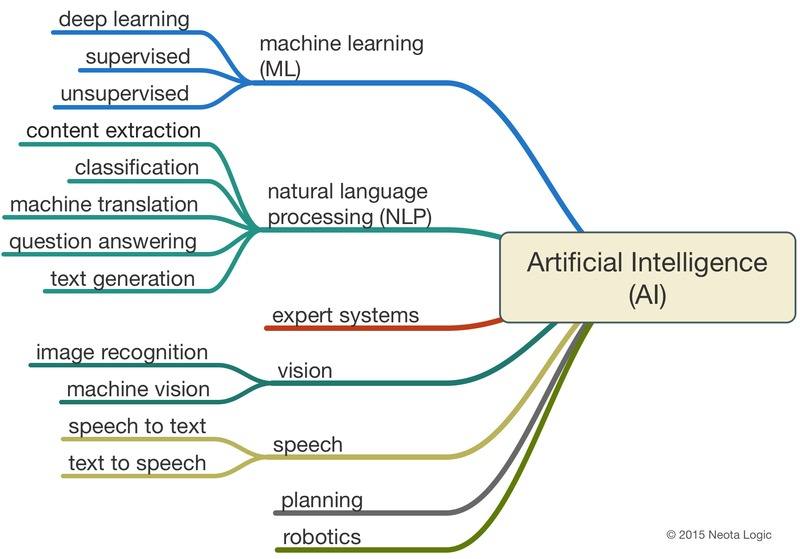
\includegraphics[width=0.7\linewidth]{images/branches}
	\end{figure}
	Pour mieux comprendre ce que sont machine learning et deep learning commençons par les \textit{systèmes experts}. Ce sont des logiciels très spécialisés dont le but est de reproduire la "pensée" d'un expert dans un domaine. Cela permet de remplacer une personne pour une tâche bien précise. Par exemple, le premier système expert mis au point, Dendral (en 1965) permettait d'identifier les consitituants chimiques d'un matériau. Les systèmes experts reposent sur des algorithmes "simples", constitués de conditions "if... then...", pouvant être assimilés à des arbres de décisions. Ils sont donc utilisables uniquement pour des tâches précises et déterminées à l'avance et ne peuvent sortir de leurs bornes d'application. L'apprentissage de la machine est manuelle, c'est l'homme qui doit implémenter toutes les possibilités lui-même.\\
	
	Le machine learning apporte une solution à cela. Dorénavant, l'ordinateur apprend par lui-même. L'homme lui apprend à reconnaitre et à reproduire. On dit qu'on "entraine" la machine. Il faut pour cela lui fournir de grands jeux de données, c'est là qu'intevient le domaine du big data et c'est une des raisons pour lesquelles le développement du machine learning s'est accéléré ces dernières années. Grâce aux données d'entraînement, le programme constitue des données statistiques sur lesquelles il s'appuie ensuite pour faire ses prévisions. \\
	
	Enfin, le deep learning est constitué d'algorithmes permettant au logiciel de s'entrainer lui même. Cette dernière approche est basée sur ce que l'on appelle des "réseaux de neurones" à multiples couches, imitant (plus ou moins) le fonctionnement du cerveau humain. Plus ils reçoivent de données, plus ces réseaux de neurones sont performants. 
	
\section{Application des algorithmes}
\chapter{Conclusion}

Ce mémoire nous a permis de faire une présentation des différentes méthodes de descente utilisées afin de résoudre différents problèmes d'optimisation et notamment de minimisation. En fonction du problème étudié et de sa dimension, nous avons un certain nombre outils à notre disposition afin de trouver le minimiseur d'une fonction. \\

Nous avons donc développé principalement l'utilisation de la méthode du gradient-conjugué ainsi que les principales caractéristiques de celle-ci. Pour ce faire, nous avons établi et défini un outil mathématique très important en minimisation : les espaces de krylov qui nous permettent de définir d'importantes propriétés de convergence pour ces algorithmes.\\

 Nous avons aussi cherché quelques pistes d'amélioration avec l'utilisation des algorithmes de Newton. Néanmoins, le calcul étant assez lourd à effectuer, nous avons exposé le principe des algorithmes de Quasi-Newton qui permettent d'approximer la matrice hessienne. Cela nous produit une famille d'algorithmes possédant les propriétés de ceux de Newton tout en étant moins lourds.\\

Ensuite, nous avons choisi d'appliquer ces études à un domaine très vaste et en expansion depuis quelques années. En effet, dès le début de notre étude des intelligences artificielles, nous nous sommes aperçus que ce n'était qu'un ensemble de mathématiques d'optimisation que nous utilisons dans différents buts. Nous avons donc appliqué cela à plusieurs problèmes. 

\appendix




%\glsaddall
%\printglossaries

%\nocite{*}

	
%	\bibliographystyle{plain} % Le style est mis entre accolades.
%	\bibliography{references} % mon fichier de base de données s'appelle bibli.bib

%\printbibliography

\listoffigures
\nopagebreak
\include{annexes}

\printindex

\end{document}